\textbf{Beispiel 1}\\ \\
a)\\ \\
Freigeschnittene Objekte
\begin{figure}[h]
	\centering
	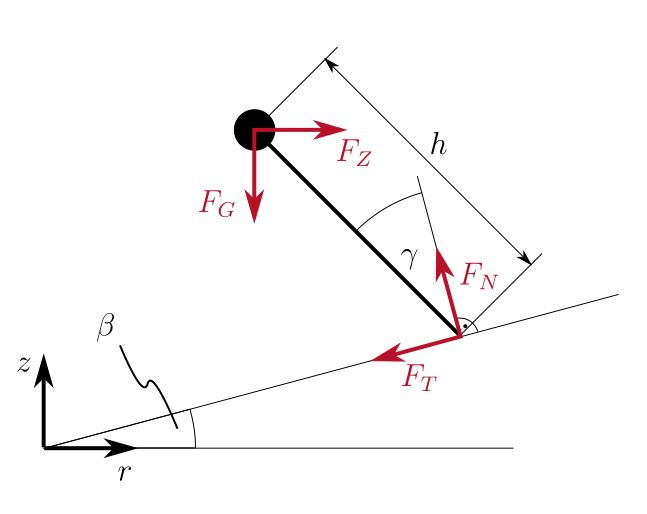
\includegraphics[width= 8cm]{tikz/30_11_2018_1a}
\end{figure}
\newline
Die wirkende Zentrifugalkraft lautet hier
\[
	F_Z = m\frac{v^2}{r_K}
\]
b) \\ \\
Die Gleichgewichtsbedingungen lauten
\begin{align*}
	\textbf{e}_x &: -F_G + F_N\cos(\beta) - F_T\sin(\beta) = 0\\
	\textbf{e}_y &: F_Z - F_N\sin(\beta) - F_T\cos(\beta) = 0\\
	\textbf{e}_z &: hF_G\sin(\beta + \gamma) - hF_Z\cos(\beta + \gamma) = 0
\end{align*}
c) \\ \\
Aus der letzten Gleichung folgt mit $F_G = mg$ und $F_Z = m\frac{v^2}{r_K}$ der Neigungswinkel
\begin{align*}
	mgh\sin(\beta + \gamma) &- m\frac{v^2}{r_K}h\cos(\beta + \gamma) = 0 \\
		g\sin(\beta + \gamma) &= \frac{v^2}{r_K}\cos(\beta + \gamma) \\
		\frac{\sin(\beta + \gamma)}{\cos(\beta + \gamma)} &= \frac{v^2}{gr_K} \\
		\tan(\beta + \gamma) &= \frac{v^2}{gr_K} \\
		\gamma &= \arctan\left(\frac{v^2}{gr_K} \right) - \beta
\end{align*}
d)\\ \\
Aus den Gleichgewichtsbedingungen folgt durch Umformen
\begin{align*}
	F_N &= F_G\cos(\beta) + F_Z\sin(\beta) \\
	F_T &= -F_G\sin(\beta) + F_Z\cos(\beta)
\end{align*}
Betrachtet man nun auch noch die Haftreibung ergibt das für die maximale Geschwindigkeit und den maximalen Neigungswinkel
\begin{align*}
	v_{max} &= \sqrt{qr_k}\sqrt{\frac{\mu + \tan(\beta)}{1 - \mu tan(\beta)}} \\
	\gamma_{max} &= \arctan\left(\frac{\mu + \tan(\beta)}{1 - \mu tan(\beta)}\right) - \beta
\end{align*}
e)\\ \\
Die Höhe des Massenschwerpunkts hat keinen Einfluss auf die maximale Geschwindigkeit, da der Neigungswinkel $\gamma$ immer derart angepasst wird, dass kein resultierendes Moment auf den Radfahrer wirkt. Die resultierende Kraft zufolge $F_G$ und $F_Z$ zeigt daher immer vom Massenschwerpunkt in Richtung Kontaktpunkt zur Fahrbahn. Der Radfahrer balanciert die auftretende Zentrifugalkraft aus.